\chapter{Clean Architecture}

%% Plugins (DB / GUI) -> Adapters (Presenters, Controllers, Gateways) -> Application Code (Use Cases) -> Domain Code (Entities) -> Abstraction Code (Generic Entities (mathematische Konzepte))
%% Abstraction Code: 
%%  Mathematische Konzepte (z.B. Matrizen)
%%  Algorithmen und Datenstrukturen (z.B. Zelluläre Automaten)
%%  Abstrahierte Muster (z.B. Quantitäten)
%%  !!!!!Häufig nicht notwendig!!!!
%% 
%% Domain Code:
%%  Entities 
%%  Implementiert organisationsweit gültige Geschäftslogik
%%  Sollte sich am seltensten ändern
%% 
%% Application Code:
%%  Use Cases
%%  Implementiert die anwendungsspezifische Geschäftslogik
%%  Steuert den Fluss der Daten und Aktionen von und zu den Entities
%% 
%% Adapters:
%%  Diese Schicht vermittelt Aufrufe und Daten an die inneren Schichten
%%  Formatkonvertierungen
%%  Oftmals nur einfache Datenstrukturen, die hin- und hergereicht werden
%%  Anti-Corruption Layer
%% 
%% Plugins:
%%  Diese Schicht greift grundsätzlich nur auf die Adapter zu
%%  Enthält Frameworks, Datentransportmittel und andere Werkzeuge (Datenbank, API)
%%  Wir versuchen, hier möglichst wenig Code zu schreiben
%%  Hauptsächlich Delegationscode, der an die Adapter weiterleitet
%% 
%% Grundregeln der Clean Architecture
%%  ● Der Anwendungs- und Domaincode ist frei von Abhängigkeiten
%%  ● Sämtlicher Code kann eigenständig verändert werden
%%  ● Sämtlicher Code kann unabhängig von Infrastruktur kompiliert und ausgeführt werden
%%  ● Innere Schichten definieren Interfaces, äußere Schichten implementieren diese
%%  ● Die äußeren Schichten koppeln sich an die inneren Schichten (Richtung Zentrum)

%% Konkrete Umsetzung
%% ●Nicht alle Klassenin einem Projekt
%% ●Schichtenbildung überPackages ist in Ordnung
%% ●Aber: keine Überprüfungdurch den Compiler
%% ●Lieber mehrere Projekte(„Multi-Projekt“)
%% ●Compiler findet nur Klassen–im eigenen Projekt–in referenzierten Projekten
%% Maven parent Pom

%% Ziel der Clean Architecture
%% Das Ziel der Clean Architecture ist, Code nur von langlebigerem Code abhängig zu machen
%% Wenn sich Technologien ändern müssen, kann die Anwendung unverändert bleiben

\section{Schichtarchitektur planen und begründen}

\begin{figure}[htbp]
    \centering
    \fbox{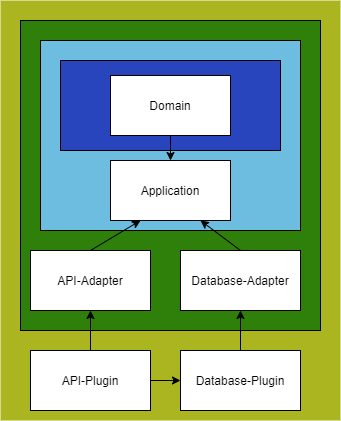
\includegraphics[width=6cm]{schichtarchitektur}}
    \caption{\label{flutter-1} Schichtarchitektur}
\end{figure}
%% genauer erklären warum es aufgespalten wurde!!!!
Die Schichtarchitektur ist in vier Schichten unterteilt: Plugin, Adapter, Application, Domain.
Die Plugin-Schicht wurde nochmals in API und Datenbank aufgeteilt um die übersichtlichkeit etwas zu erhöhen.
Dementsprechend wurde die Adapter-Schicht auch in API und Datenbank aufgeteilt und konvertiert die jeweiligen Objekt-Formate in die Formate der inneren Schichten.
Die Adapter rufen dann Funktionen aus der Application Schicht auf.
In der Application-Schicht liegt dann die eigentliche Logik der Anwendung und hier werden API und Datenbank zusammen geführt.
In der Domain Schicht befinden sich die Entities und Value Objects der Application Schicht,
dies dient dem Ziel diese in Zukunft in weiteren Application-Schichten einheitlich verwenden zu können.
Zusätzlich enthält die Domain Schicht die Repository-Interfaces welche von darunter liegenden Schichten implementiert werden um eine Inversion of Control zu erzeugen.
%% fundamental: von aussen nach innen!!!!!!!
%% TODO vlt bisschen mehr schreiben, Begründung fehlt
%% Anwendung macht xy
%% ich ordne folgende funktionen der folgenden Schicht zu ...
%% die sind da weil ...
%% Folgende schichten wurden nicht verwendet weil....